\section{Usage Examples}\label{sec:usage}
\todo{Pick two Kaggle examples and show how \system implements those.}

\stitle{Tweet analysis.} Notebook workflow does exploratory analysis by visualizing parts of the initial dataset using different barchart/histogram visualizations. They do data cleaning and then create a model using GloVe for vectorization and keras for building the model. The model is a classifier that determines whether the tweet is a disaster or not.

\stitle{Spam detection.} Notebook workflow does initial exploratory analysis, cleaning/pre-processing, building the model, and then doing a visualization of the resulting confusion matrix as a heatmap. The SMS Spam Collection contains one set of SMS messages in English of 5,574 messages, tagged according being ham (legitimate) or spam. This corpus has been collected from free or free for research sources from the Internet. The aim to correctly predict a given piece of text as Spam or Ham.


% \begin{figure*}[!htb]
% \centering
% \begin{tabular}{ c c c}
%   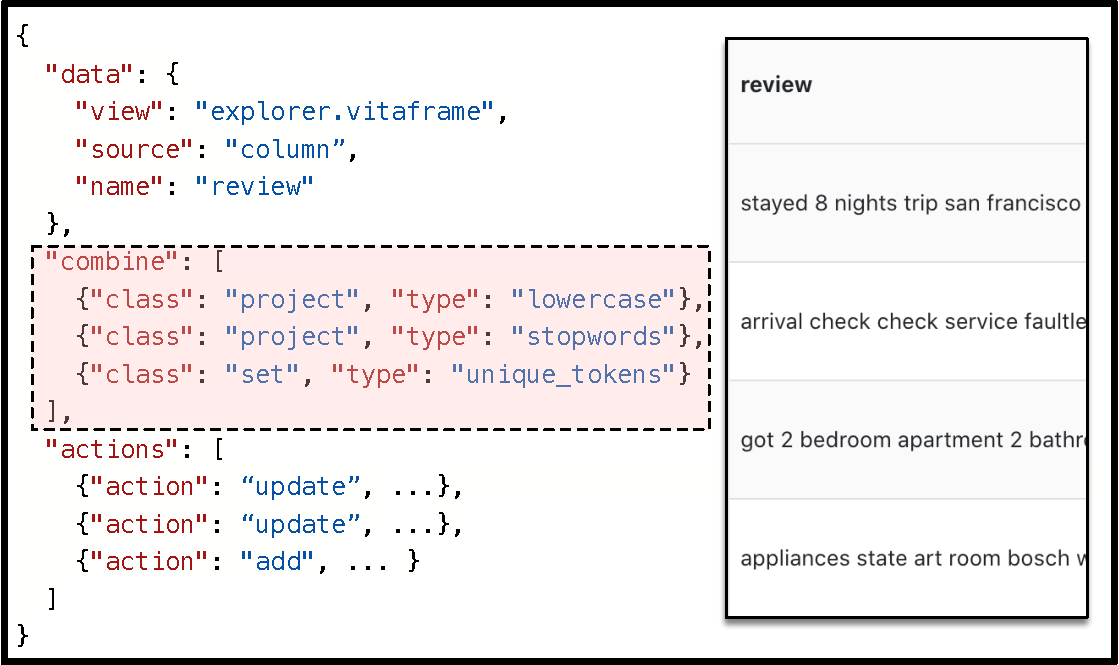
\includegraphics[width=0.3\linewidth,height=0.18\linewidth]{figures/combine_clean.pdf}   & 
%   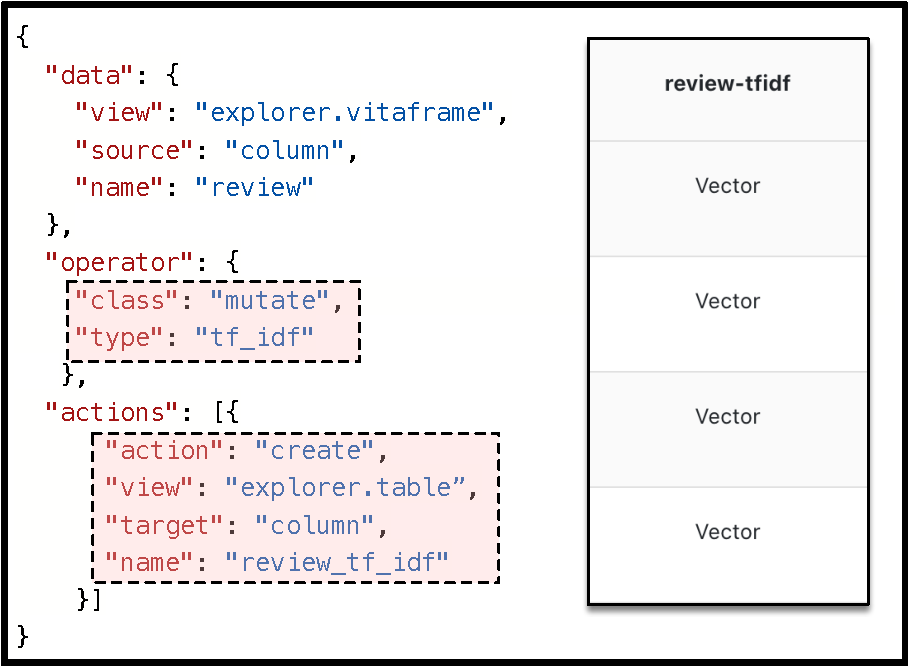
\includegraphics[width=0.3\linewidth,height=0.18\linewidth]{figures/tf_idf.pdf} & 
%   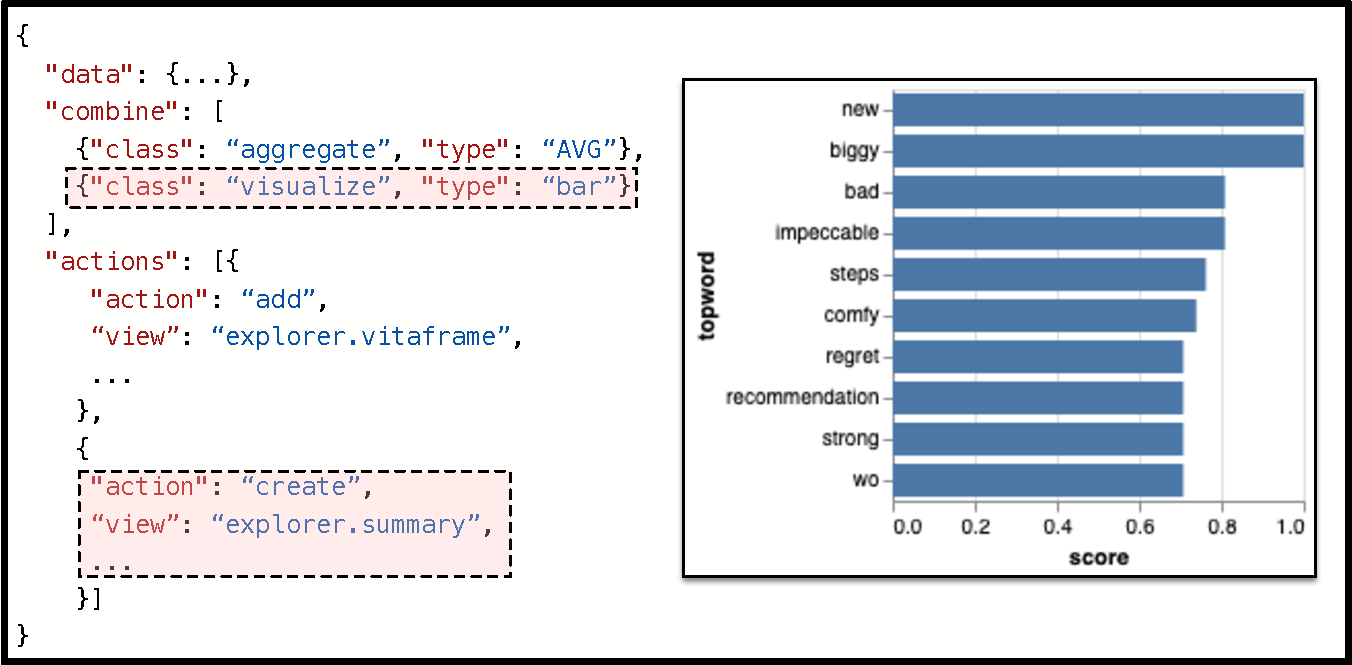
\includegraphics[width=0.3\linewidth,height=0.18\linewidth]{figures/barchart.pdf} \\
%      (a) Clean and generate metadata & 
%      (b) Create TF-IDF feature vector &
%      (c) Visualize top-words by TF-IDF score
% \end{tabular}
%     \caption{Example of \vta specification. (a) Use \emph{Combine} operator to clean data (\eg \emph{lowercasing}, \emph{stopwords removal}) and generate metadata (\eg \emph{unique\_token} to create token dicitionary) for use in subsequent steps. (b) Define featurization operation and subsequent action, \ie column creation in table view. (c) Compute average TF-IDF score of each token in the dictionary using \emph{aggregate} operator and then create barchart of top-ranked words using \emph{visualize} operator.}
% \vspace{-15pt}
%     \label{fig:use-case-a}
% \end{figure*}

% \begin{figure*}[tbp]
% \centering
% \small
% \begin{tabular}{ c c}
%   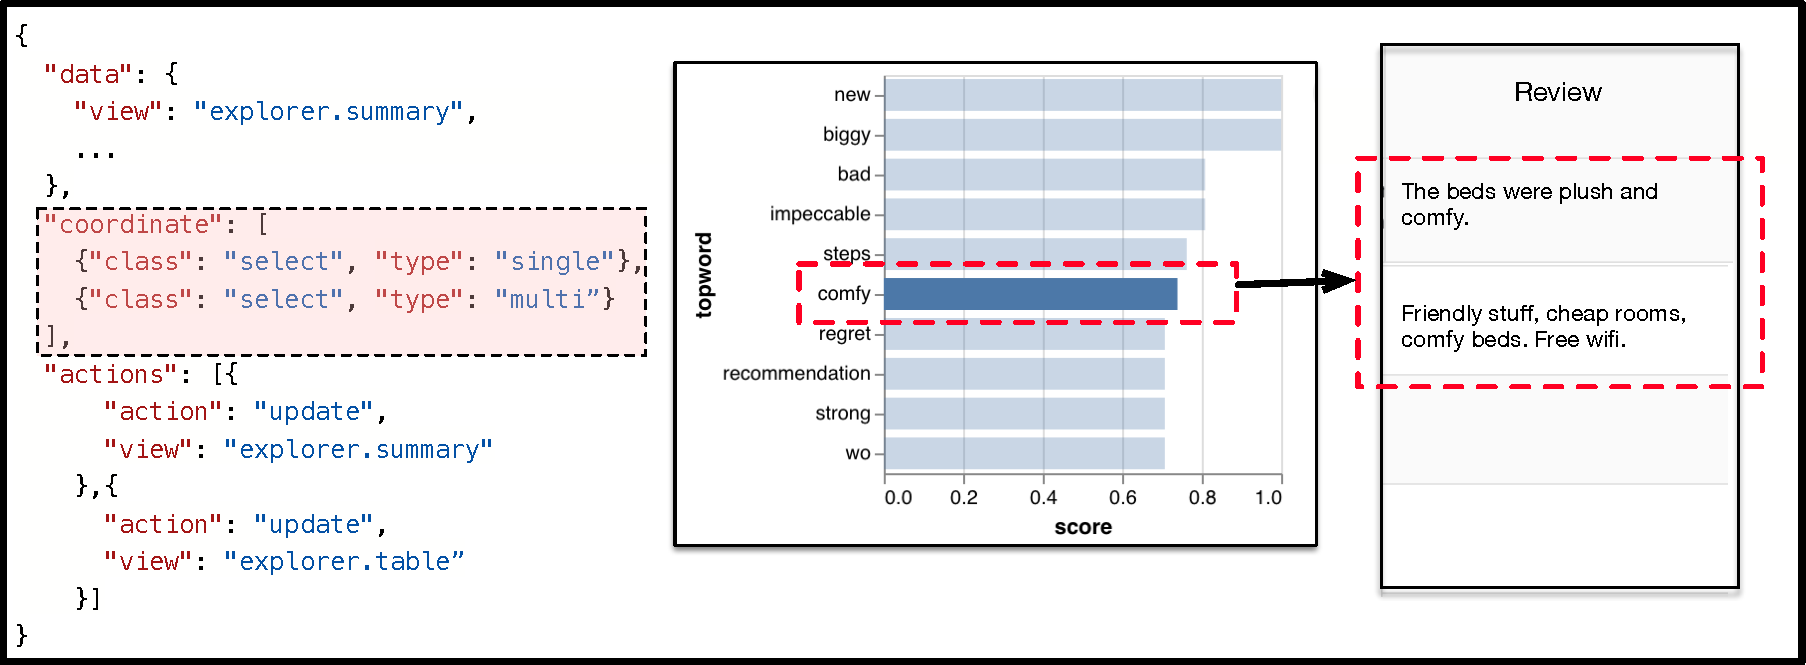
\includegraphics[width=0.5\linewidth,height=0.18\linewidth]{figures/unidirect_bar_table.pdf}   & 
%   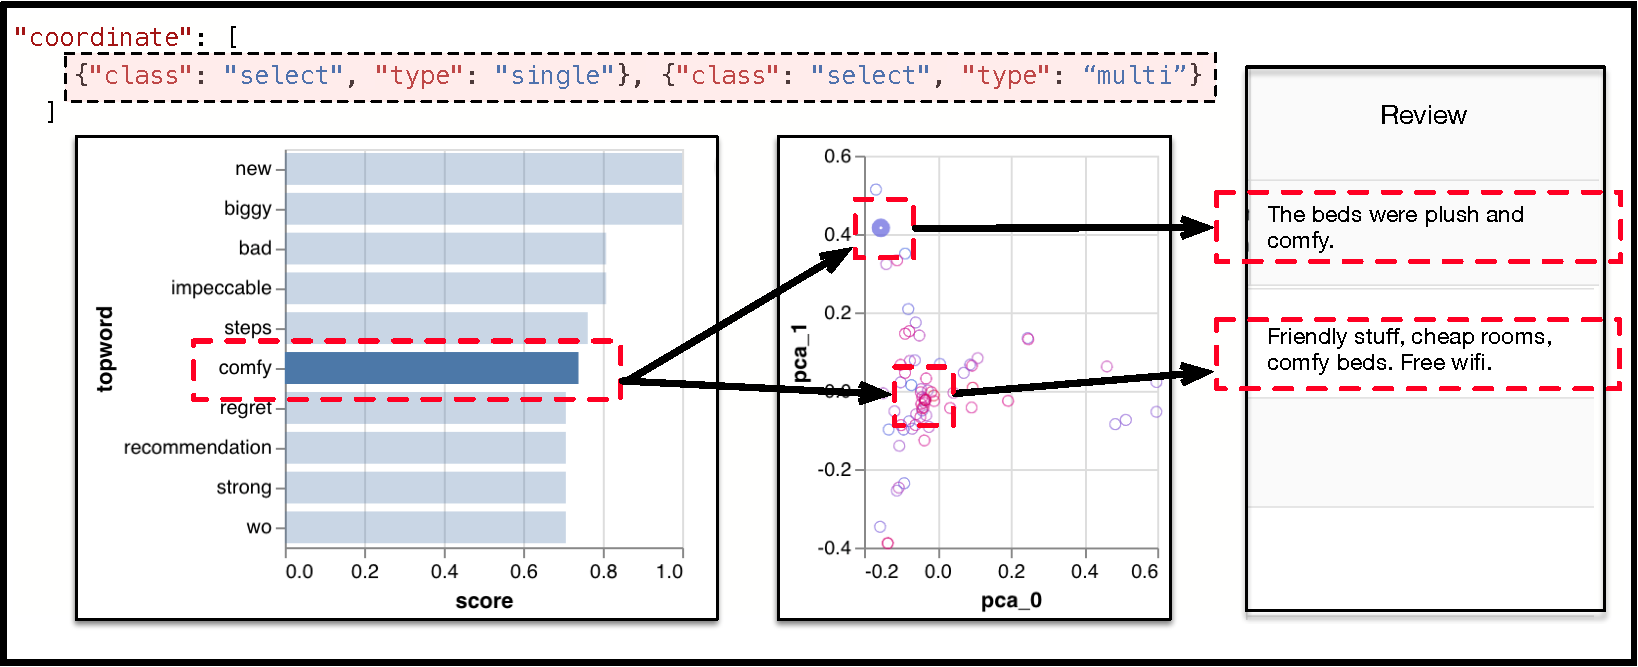
\includegraphics[width=0.5\linewidth,height=0.18\linewidth]{figures/unidirect_bar_table_scatter.pdf} \\
%      (a) Coordination of two views & 
%      (b) Coordination of three views 
% \end{tabular}
%     \caption{\small Multi-view coordination. (a) Use the \code{coordinate} operator to link the bar chart and Table View. Selecting a bar (word) in the bar chart triggers a \code{filter} by the selected word on Table View . (b) Coordinating the bar chart and scatterplot links the three views. Selecting a bar in the bar chart highlights relevant points in the scatterplot, and filters relevant rows in Table View.}
%     \label{fig:use-case-b}
%     \vspace{-15pt}
% \end{figure*}
